\documentclass{itatnew}

\usepackage{paralist} % inparaenum support
\usepackage{varioref} % added by Viliam for \vref
\usepackage{xcolor} % added by Viliam for \textcolor

\usepackage{caption}
\usepackage{subcaption}
\usepackage{graphicx}
\usepackage{textcomp} % used for degrees celsius
\usepackage{booktabs}
\usepackage[british]{babel}

% ==========================================
% Support for \FOCAL{R}{M}{op} (by Viliam)
% ==========================================
\newcommand{\FOCALMMODE}[3]{
  #1{\stackrel{\mathtt{#3}}{\circ}}#2
}
\newcommand{\FOCAL}[3]{
  \ifmmode
  \FOCALMMODE{#1}{#2}{#3}
  \else
  \begin{math}\FOCALMMODE{#1}{#2}{#3}\end{math}%
  \fi
}
% ==========================================

\begin{document}

\title{Stable Hot Spot Analysis (Draft)}

\author{
  Marc Gassenschmidt \and
  Viliam Simko  \and
  Julian Bruns
  \\
  \email{todo@fzi.de},
  \email{simko@fzi.de},
  \email{bruns@fzi.de}
}

\institute{
  FZI Forschungszentrum Informatik\\
  am Karlsruher Institut f\"ur Technologie\\
  76131, Haid-und-Neu-Str. 10-14\\
  Karlsruhe, Germany
}
  
\maketitle              % typeset the title of the contribution



\begin{abstract}
Hotspot analysis is an essential in geo-statistics. It supports decision making by detecting points as well as areas of interest in comparison to their neighbourhood. But these methods are dependent on different parameters, ranging from the resolution of the study area to the size of their neighbourhood. This dependence can lead to instabilities of the detected hotspots, where the results can highly vary between different parameters. A decision maker can therefore not be sure of the validity of analysis. In this study, we examine the impact of key parameter on the stability of the hotspots, namely the size of the neighbourhood (blurr), the resolution (zoom) and the size of the study area, as well as the influence of the ratio between those parameter. We compute the hotspots with the well known Getis-Ord ($G^*$) statistic as well as an modification, the \emph{Focal $G^*$} statistic. The stability of the hotspot analysis is measured with the recently introduced \emph{stability of hotspots} (SoH) metric and by visual analysis. We evaluate the results on real world data with the well-known yellow cab taxi data set from New York, Manhattan. It can be shown that 
   
\end{abstract}


\section{Introduction}

For urban city planers, the detection of Intra Urban Heat Islands (IUHI) is of
high interest as high temperatures impact energy
consumption~\cite{Hassid.2001.Electricity_UHI} as well as human
health~\cite{Ye.2012}. The effect that the temperatures between an urban area
and its surroundings differ, called the Urban Heat Island effect
\cite{Oke1982energetic}, has long been the subject of research. Most historical
studies conducted had to rely on few, fixed weather stations, low
spatio-temporal resolution of satellites or small-scale mobile measurements by
car, preventing the modelling of finer-grained temperature differences within an
urban area itself. With the advent of inexpensive mobile sensors, higher
spatio-temporal resolution of satellites and volunteered geographic
informations, to name just a small selection, it is now feasible to focus on the
temperature differences in a city as the subject of interest.

Hot spot analysis is a tool which is suited to detect such areas. In the context
of IUHI we can detect those areas where the temperature is significantly
different from the mean temperature of our study area. This enables us to
identify points of interest without the need to pre-process the data.

Although existing methods are independent of concrete values, their results are
highly dependent on the size of the study area and their parametrization such as
the weight matrix in the case of the Getis-Ord statistic. This dependency can
lead to unstable hot spots, where the identified hot spots only appear in one 
specific combination of parameter. The generalization of insights gained from
unstable hot spots is suboptimal. A city planer who has to rely on those
insights will most likely prioritize the wrong area to invest his limited
resources. Given the increasing importance to detect extreme local temperatures
in cites, see e.g. \cite{Hansen.2010, GRL:GRL22143, department2014world}, means
to reliably detect and mitigate the effect of temperature extremes in a
proactive fashion are needed.

To solve this problem, we first propose a metric to measure the stability of a
hot spot analysis regarding its parametrization of the weight matrix called the
\emph{Stability of Hot spot} (SoH). This metric measures whether a hot spot
found for a given weight matrix is carried over to the found hot spots with a
different weight matrix. This enables us to quantify the stability of any hot
spot analysis. Based on our reasoning behind the instability of existing hot
spot analyses, we propose a modification of the well known Getis-Ord statistic
($G^*$): the \emph{Focal Getis-Ord} statistic (Focal $G^*$). Instead of the
global mean and variance used by $G^*$, it only uses the mean and variance of a
predefined region around each point. This region is a subset of the whole study
area. By doing this, the instability is contained within a smaller region and
thereby independent of the parametrization of the weight matrix. We test our
stability metric as well as this modified approach on data given by two
temperature snapshots of the city of Karlsruhe taken in 2008.

\section{Related Work}

\subsection{Urban Heat Island}

The scientific interest in the phenomena of UHI is well established. One of the
earliest known overviews of the scientific literature of the city climates is
given by Albert Kratzer 1937~\cite{dieckmann1938stadtklima}. At that time
already, relations between temperature, humidity, human heat fluxes and air
pollution are investigated.

A more recent overview comes from Arnfied~\cite{Arnfield.2003}. The focus here
lies on the development in the field of climatology between 1980 and 2003. In
particular, the rise of simulations and modelling is lauded, but, to quote
Arnfield, ``simple methods are still needed to estimate UHI intensity within
urban areas''~\cite{Arnfield.2003}.

Schwarz~et~al.~\cite{Schwarz.2011} compare 11 different Surface Urban Heat
Island (SUHI) indicators on a dataset of 263 European cities with monthly mean
temperatures. They show that the selection of indicators is important for the
detection of UHI due to possible instabilities of each indicator.

A more recent development is the focus on IUHI. The definition for IUHI comes
from Martin et al.~\cite{Martin.2015}. By defining thresholds with respect to
spatial reference, these enable the detection of hot spots in a city, which
Martin et al. call surface intra-UHI. This boils down to five steps, i.e.
essentially a comparison of absolute deviation from the mean temperature given a
survey area. The results can then be used to detect areas of interest in a city
and potentially trigger alerts for a much finer spatial granularity.

While the proposition to examine urban micro-climates can be traced back as far
as 1937~\cite{dieckmann1938stadtklima}, we have found only few works in this
field. Schwarz et al.~\cite{Schwarz.2012} state that the reduction of an UHI to
a single value for a whole city is questionable regarding its explanatory power.
But also that there is currently no other way to quantify the differences
amongst cities.

The difficulties presented by comparing the UHI values between different cities
are the topic of Stewart and Oke~\cite{Stewart2012}. They propose the use of
local climate zones (LCZ) to standardise the methodology and terminology.

Another area where urbanizations affects the temperature distribution are
subsurface temperatures. Menberg et al.~\cite{Menberg.2013} look into the
distribution of the temperatures below the surface -- the subsurface
temperature. They find local hot spots of heat with deviations of up to
+20\textdegree{K} in some areas related to local heat sources.

\subsection{Hot Spot Analysis}

The goal of an analysis of temperatures in a city is to find the most
interesting, significant areas: Hot spots~\cite{Martin.2015}. This goal is
similar to the hot spot analysis in the field of geo-statistics. One of the most
fundamental approach is Moran´s I~\cite{MoranI}. There it is tested whether or
not a spatial dependency exists. This gives the information on global
dependencies in a data set. Upon this hypothesis test several geo-statistical
tests are based. The most well known are the Getis-Ord statistic~\cite{Ord.1995}
and LISA~\cite{Anselin.1995}. In both cases the general, the global statistic of
Moran´s I is applied in a local context. The goal is to detect not only global
values, but instead to focus on local hot spots and to measure the significance
of those local areas.

The local Getis-Ord statistic~\cite{Ord.1995} is defined as follow:
\begin{definition}[Getis-Ord $G^*_i$ statistic] \label{def:Gstar}
  Assuming a study area with $n$ measurements, let $X = [x_1, \ldots,
  x_n]$ be all values measured in this area. Let $w_{i,j}$ be a spatial weight
  between two points $i$ and $j$ for all $i,j \in \{ 1, \ldots, n\}$. The 
  Getis-Ord $G^*_i$ statistic is given as:
  \begin{equation} \label{eq:Gstar}
  G^*_i = \frac{
    \sum_{j=1}^{n}w_{i,j}x_j - \bar{X}\sum_{j=1}^{n}w_{i,j}
  }{
  S \sqrt{
    \frac{
      n \sum_{j=1}^{n}w_{i,j}^2 - (\sum_{j=1}^{n}w_{i,j})^2
    }{n-1}
  }
}
\end{equation}
where:
\begin{itemize}
  \item $\bar{X}$ is the mean of all measurements,
  \item $S$ is the standard deviation of all measurements.
\end{itemize}
\end{definition}

As it is known, this statistic creates a z-score, which denotes the significance
of an area in relation to its surrounding areas.

LISA is quite similar, as it is the local statistic for Moran's
I~\cite{Anselin.1995}, but the z-score has a different meaning. Apart from
$G^*_i$, LISA does not distinguish between cold spots and hot spots as it
assigns high z-score to most similar areas.

Two other well known method are the kernel density estimation~\cite{KDE_Hotspot}
and kriging~\cite{Kriging_Hotspot}. These do not provide significance levels.
Instead, they estimate the values for each location based on the rest of the
study area and a threshold value \cite{Thakali2015}. Therefore, results for
different areas are not comparable, especially in the case of differing
temperature distributions. Kriging was developed for the estimation of ore
deposits~\cite{krige1951statistical}, but today, applications for geo-temporal
forecasts with this approach can be found, e.g. for the city of
Zurich.~\footnote{https://r-video-tutorial.blogspot.de/2015/08/spatio-temporal-kriging-in-r.html}

All of the aforementioned methods use weights between pairs of points, usually
based on their geographical distance. However, in real applications, the points
are aggregated into rasters and the weights are represented as a weight matrix.
This allows for expressing the algorithms in terms of map algebra operations, a
term first coined by Dana~Tomlin~\cite{Tomlin1990} and computed in a distributed
fashion (e.g. using Geotrellis framework running on
Apache~Spark~\cite{github:Geotrellis}).

In this work, we focus on the Getis-Ord statistic applied to rasters of land
surface temperature. This enables us to transform the formula for the $G^*$
statistic into a computationally more efficient form. We then propose a
modification of the standard $G^*$ statistics, to increase the stability of the
hot spots found.

\section{Stability of Hot Spot Analysis}
\label{sec:Metric}

Existing methods to determine hot spots are dependent on the parametrization of
the weight matrix as well as on the size of the study area.

Consider the real-world example depicted in Fig.~\ref{fig:TempMaps}. The
temperature map of a morning thermal flight dataset (Fig.~\ref{fig:TempMaps:a})
has been processed using $G^*$.

\begin{figure}[htp]
  \begin{subfigure}{1\linewidth}
    \caption{Morning temperatures}
    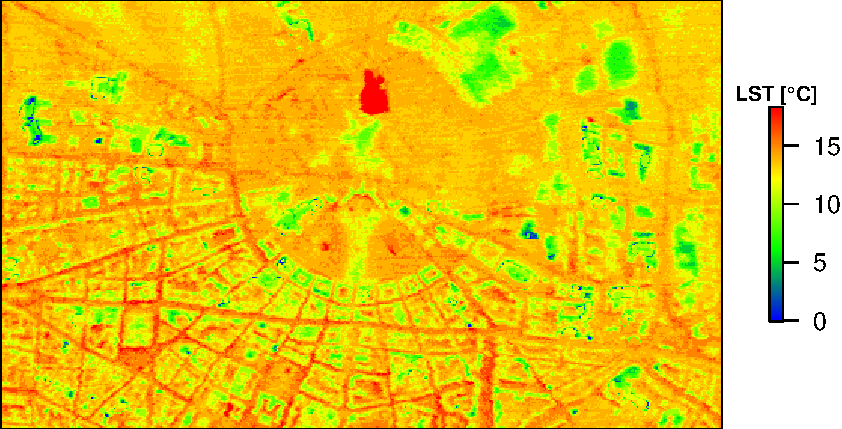
\includegraphics[width=\linewidth]{images/hotspot-rawtemp-1}
    \label{fig:TempMaps:a}
  \end{subfigure}
  
  \caption{
    Karlsruhe city center.
    Selected area of $2.4{\times}1.4\,km$.
    Pixel size $5{\times}5\,m$.
  }
  \label{fig:TempMaps}
\end{figure}

% Bild besteht aus orginal, weight matrix a und weight matrix b
As we can see, hot spots are oftentimes disappearing or appearing unrelated to
previously found hot spots. While these computations indeed show hot spots and
the results are correct, they lack stability.

For a data analyst, when exploring the data interactively by choosing different
filter sizes (in form matrices), it is important that the hot spot's position
and size changes in a predictable manner. This intuition is the basis for our
stability metric.

We define a hot spot found in comparably more coarse resolutions as
\emph{parent} (larger weight matrix) and in finer resolutions as \emph{child}
(smaller weight matrix). To be stable, one assumes that every parent has at
least one child and that each child has one parent. For a perfectly stable
interaction, it can be easily seen that the connection between parent and child
is a injective function and between child and parent a surjective function. To
measure the closeness of connection, we propose a metric called the
\emph{Stability of Hot spot} (SoH). It measures the deviation from a perfectly
stable transformation of resolutions.

%TODO: what about the other direction?
In its downward property (from parent to child, injective) it is defined as:
\begin{equation}
\label{eq:SoH-down}
SoH^\downarrow = \frac{ParentsWithChildNodes}{Parents} = \frac{|Parents \cap 
Children|}{|Parents|}
\end{equation}
And for its upward property (from child to parent, surjective):
\begin{equation}
\label{eq:SoH-up}
SoH^\uparrow = \frac{ChildrenWithParent}{Children} = 1 - \frac{|Children - 
Parents|}{|Children|}
\end{equation}
where $ParentsWithChildNodes$ is the number of parents that have at least one 
\emph{child}, $Parents$ is the total number of \emph{parent}, 
$ChildrenWithParent$ is the number of children and $Children$ as the total 
number of children.
The SoH is defined for a range between 0 and 1, where 1 represents a perfectly 
stable transformation while 0 would be a transformation with no stability at 
all.

\section{Focal Getis-Ord} \label{sec:FocalGetisOrd}

\subsection{Dataset}

% extent
The two datasets (morning and evening flights) depicted in
Fig.~\ref{fig:ComparisonMorning} and Fig.~\ref{fig:ComparisonEvening} were
obtained from a thermal flight over the city of Karlsruhe on 26.09.2008 at
6:30--7:45 and 20:00--21:30. The flights were executed by the
Nachbarschaftsverband
Karlsruhe\footnote{http://www.nachbarschaftsverband-karlsruhe.de/}. A single
pixel in the raster represents an area of approximately $5{\times}5m$. The whole
dataset of size $35{\times}25\,km$ was cropped into the inner city area of
$2.4{\times}1.4\,km$. % temp range
The temperatures in our dataset range from -1.7°C to 18.3°C.
% missing values = NAs
Missing values in the dataset were interpolated using a focal median function
with a square matrix of 11x11 pixels, mainly for speeding up further
computations and to avoid special handling of NA values.


\subsection{Method}

In the following text, we use the notation \FOCAL{R}{M}{op} to denote
a focal operation $op$ applied on a raster $R$ with a focal window determined 
by a
matrix $M$. This is rougly eqivalent to a command \verb|focal(x=R, w=M, fun=op)|
from package \emph{raster} in the R programming language \cite{cran:raster}.

\begin{definition}[$G^*$ function on rasters]
  \label{def:GenericGetisOrdFunc}
  
  The function $G^*$ can be expressed as a raster operation:
  
  \begin{displaymath}
  G^*(R, W, st) =
  \frac{
    \FOCAL{R}{W}{sum} - M*\sum_{w \in W}{w}
  }{
  S \sqrt{
    \frac{
      N*\sum_{w \in W}{w^2} - (\sum_{w \in W}{w})^2
    }{
    N - 1
  }
}
}
\end{displaymath}
\noindent where:
\begin{itemize}
  
  \item $R$ is the input raster.
  
  \item $W$ is a weight matrix of values between 0 and 1.
  
  \item $st = (N, M, S)$ is a parametrization specific to a particular version
  of the $G^*$ function. (Def.\vref{def:StdGetisOrdVersion} and
  \vref{def:FocalGetisOrdVersion}).
  
\end{itemize}
\end{definition}

\begin{definition}[Standard $G^*$ parametrization]
  \label{def:StdGetisOrdVersion}
  
  Computes the parametrization $st$ as global statistics for all pixels in the
  raster $R$:
  
  \begin{itemize}
    \item $N$ represents the number of all pixels in $R$.
    \item $M$ represents the global mean of $R$.
    \item $S$ represents the global standard deviation of all pixels in $R$.
  \end{itemize}
\end{definition}

\begin{definition}[Focal $G^*$ parametrization]
  \label{def:FocalGetisOrdVersion}
  
  Let $F$ be a boolean matrix such that: $all(dim(F) \geq dim(W))$.
  This version uses focal operations to compute per-pixel statistics given by 
  the focal neighbourhood $F$ as follows:
  
  \begin{itemize}
    
    \item $N$ is a raster computed as a focal operation \FOCAL{R}{F}{sum}. Each
    pixel represents the number of pixels from $R$ convoluted with the matrix
    $F$. 
    
    \item $M$ is a raster computed as a focal mean \FOCAL{R}{F}{mean}, thus each
    pixel represents a mean value of its $F$-neighbourhood.
    
    \item $S$ is a raster computed as a focal standard deviation
    \FOCAL{R}{F}{sd}, thus each pixel represents a standard deviation of its
    $F$-neighbourhood.
    
  \end{itemize}
  
\end{definition}

\section{Results}
\subsection{Heatmap}
\begin{figure}[htp]
  \begin{subfigure}{\linewidth}
    \caption{FocalRelation}
    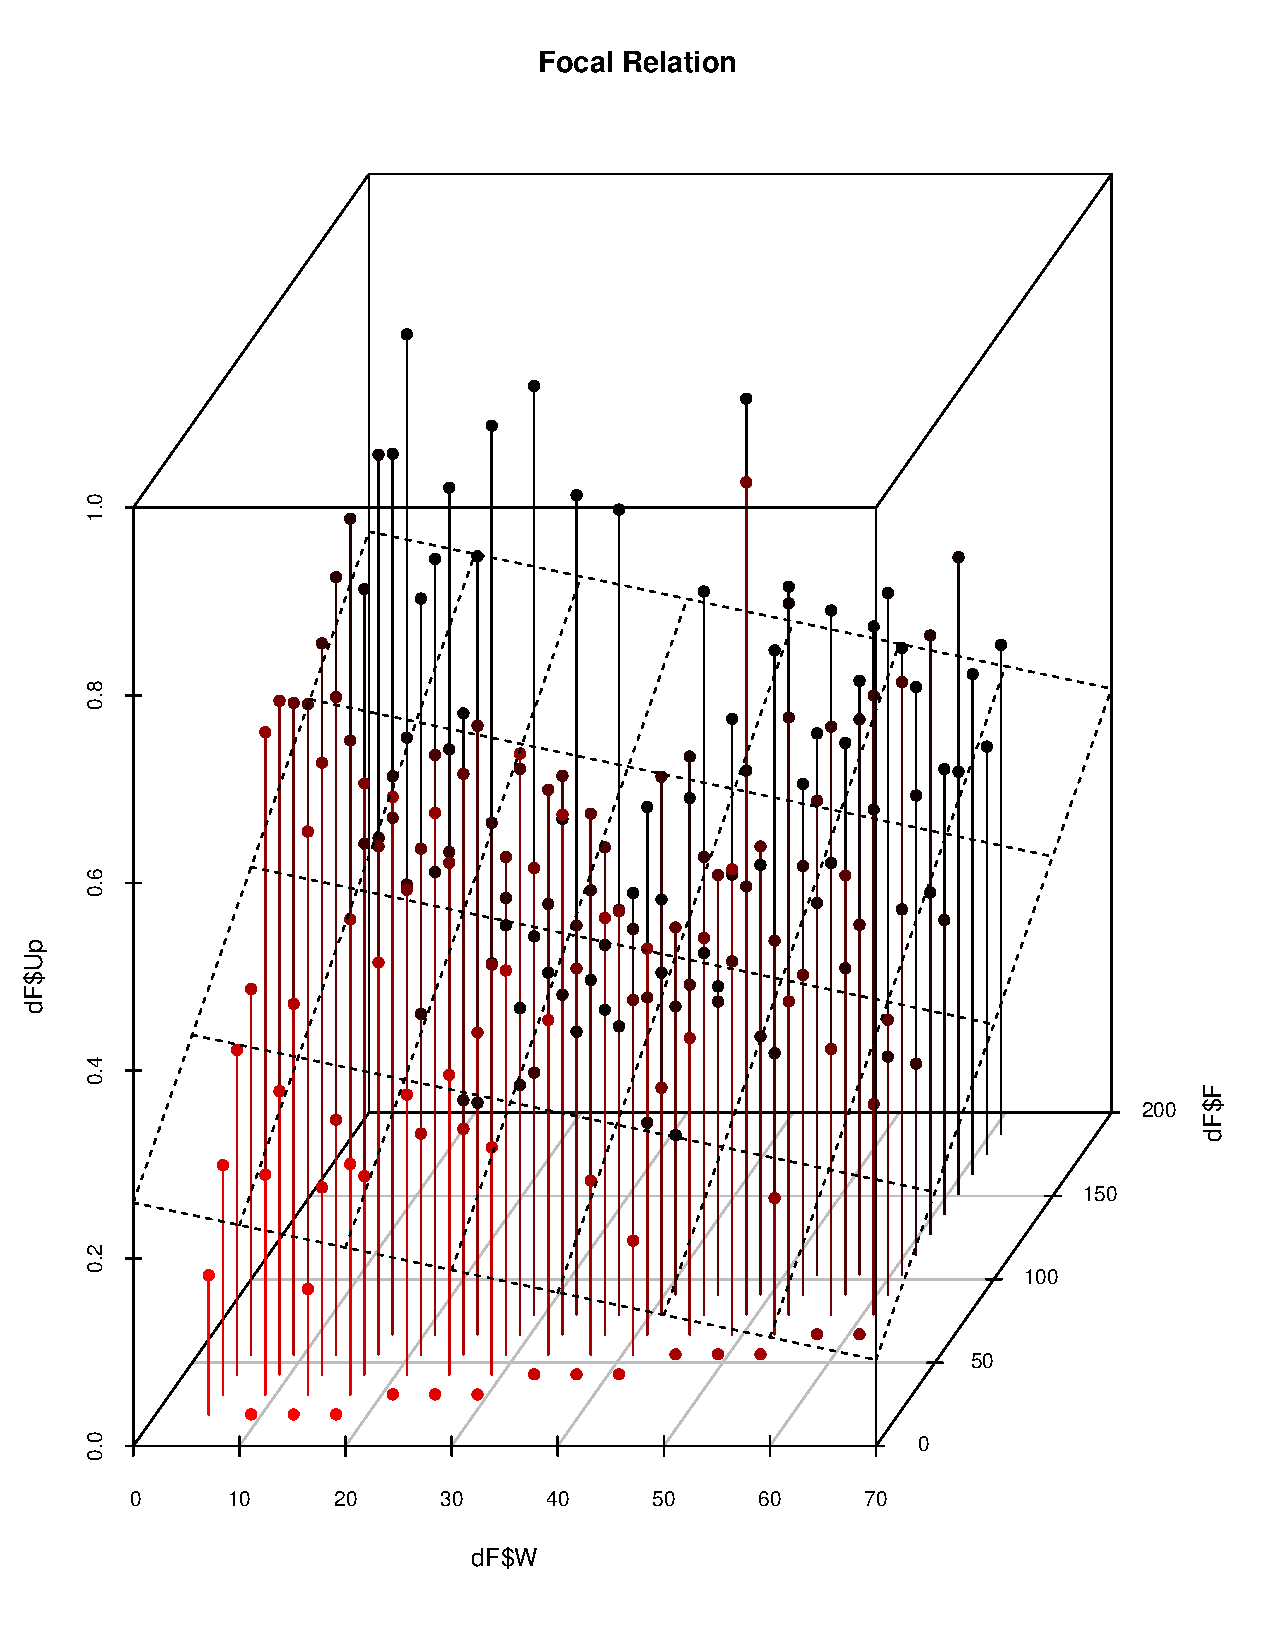
\includegraphics[width=\linewidth]{images/FocalRealationUp}
    \label{fig:FocalRelation}
  \end{subfigure}
  \hspace{1em}
  \begin{subfigure}{\linewidth}
    \caption{WeightRealtion}
    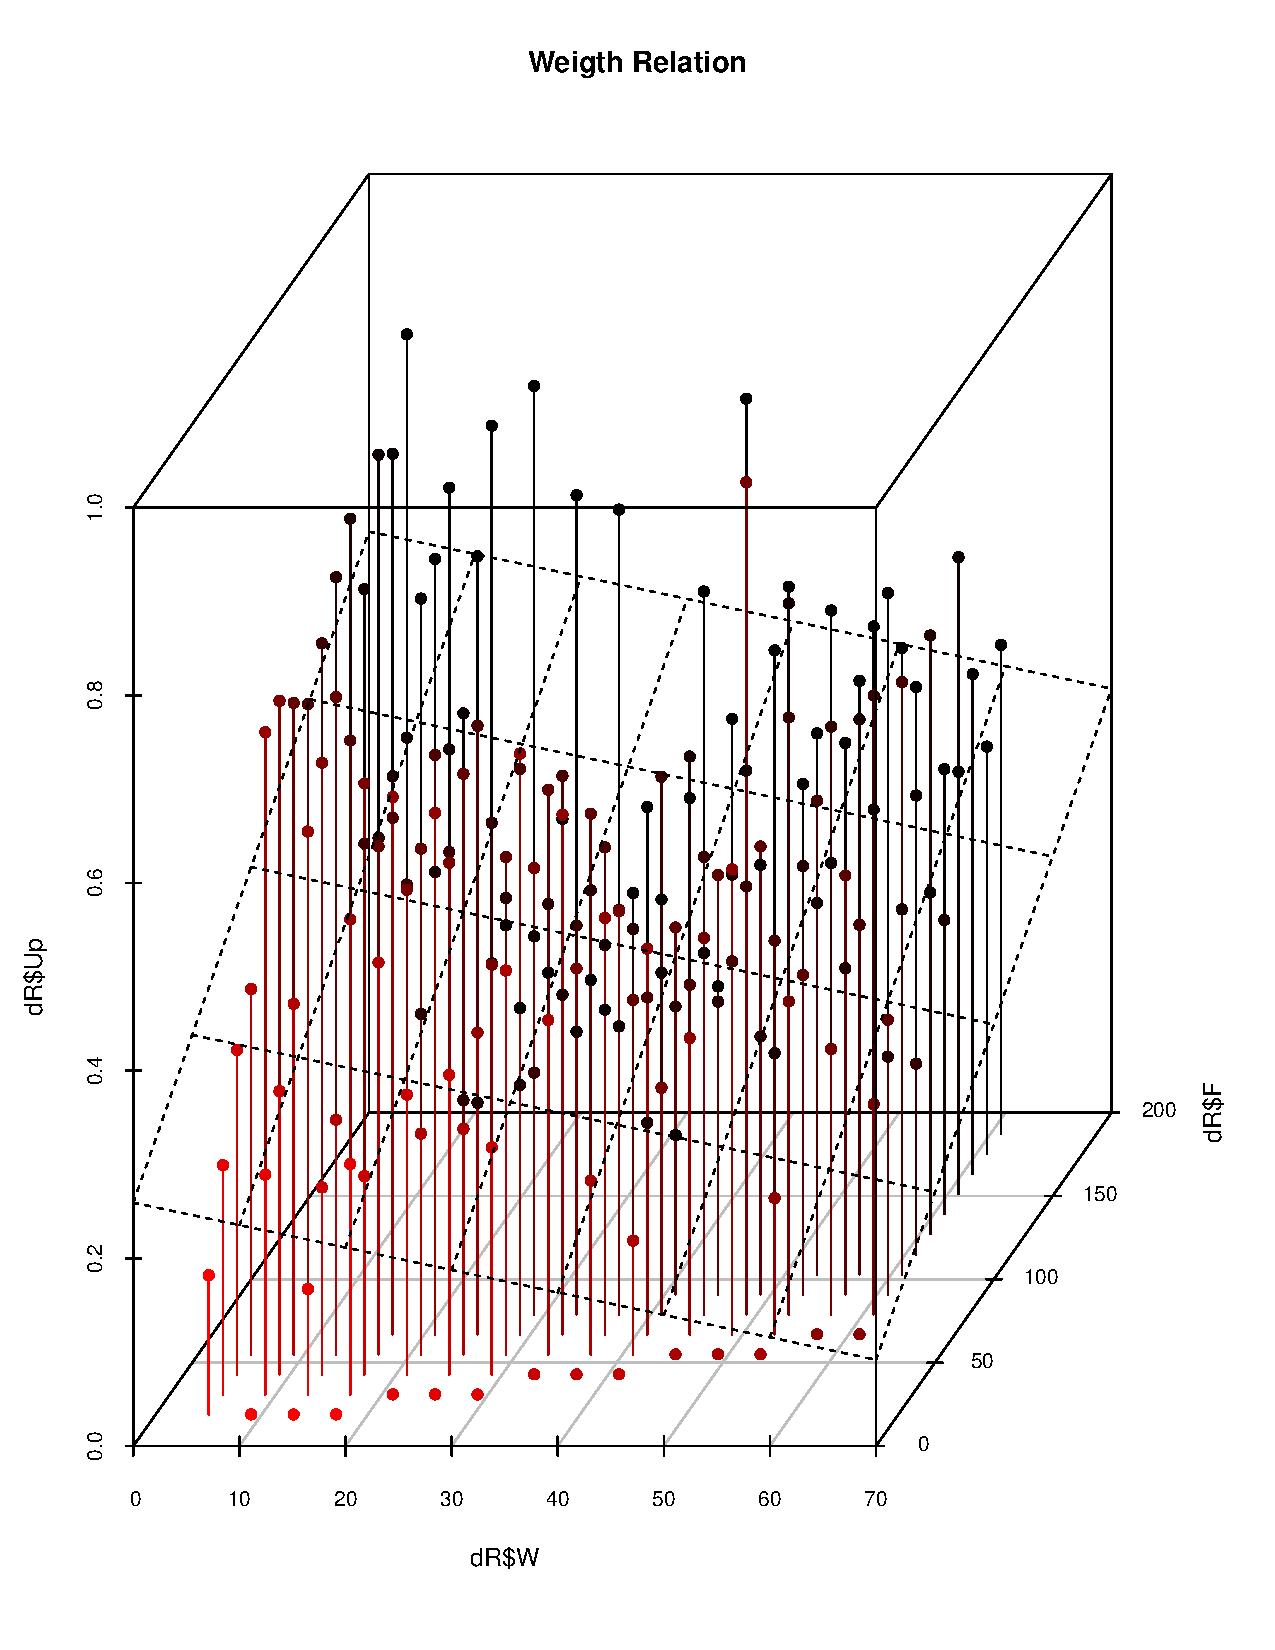
\includegraphics[width=\linewidth]{images/WeightRelationUp}
    \label{fig:WeightRealtion}
  \end{subfigure}
  \caption{Heatmap of Relation between size of weight matrix $W$ and focal matrix $F$}
  \label{fig:RealtionUp}
\end{figure}

\begin{figure}[htp]
  \begin{subfigure}{\linewidth}
    \caption{FocalRelation}
    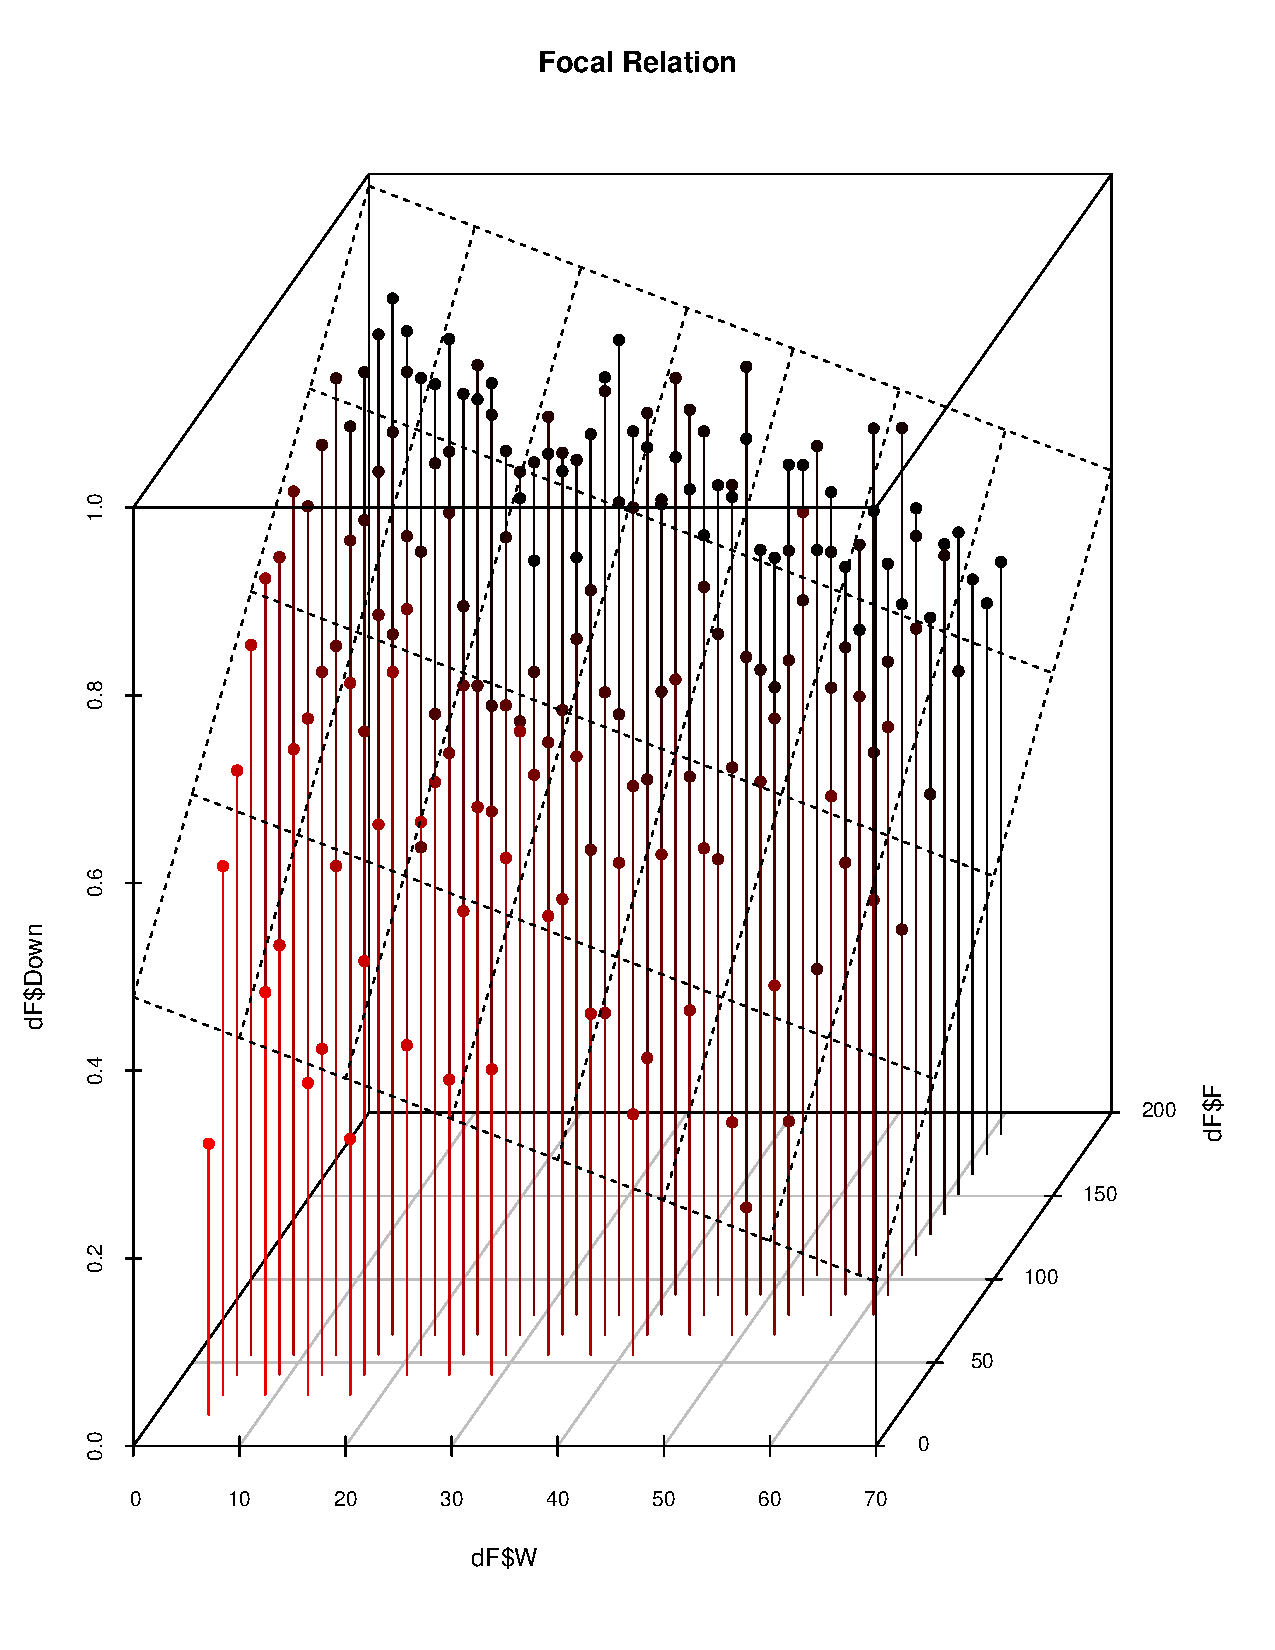
\includegraphics[width=\linewidth]{images/FocalRealationDown}
    \label{fig:FocalRelation}
  \end{subfigure}
  \hspace{1em}
  \begin{subfigure}{\linewidth}
    \caption{WeightRealtion}
    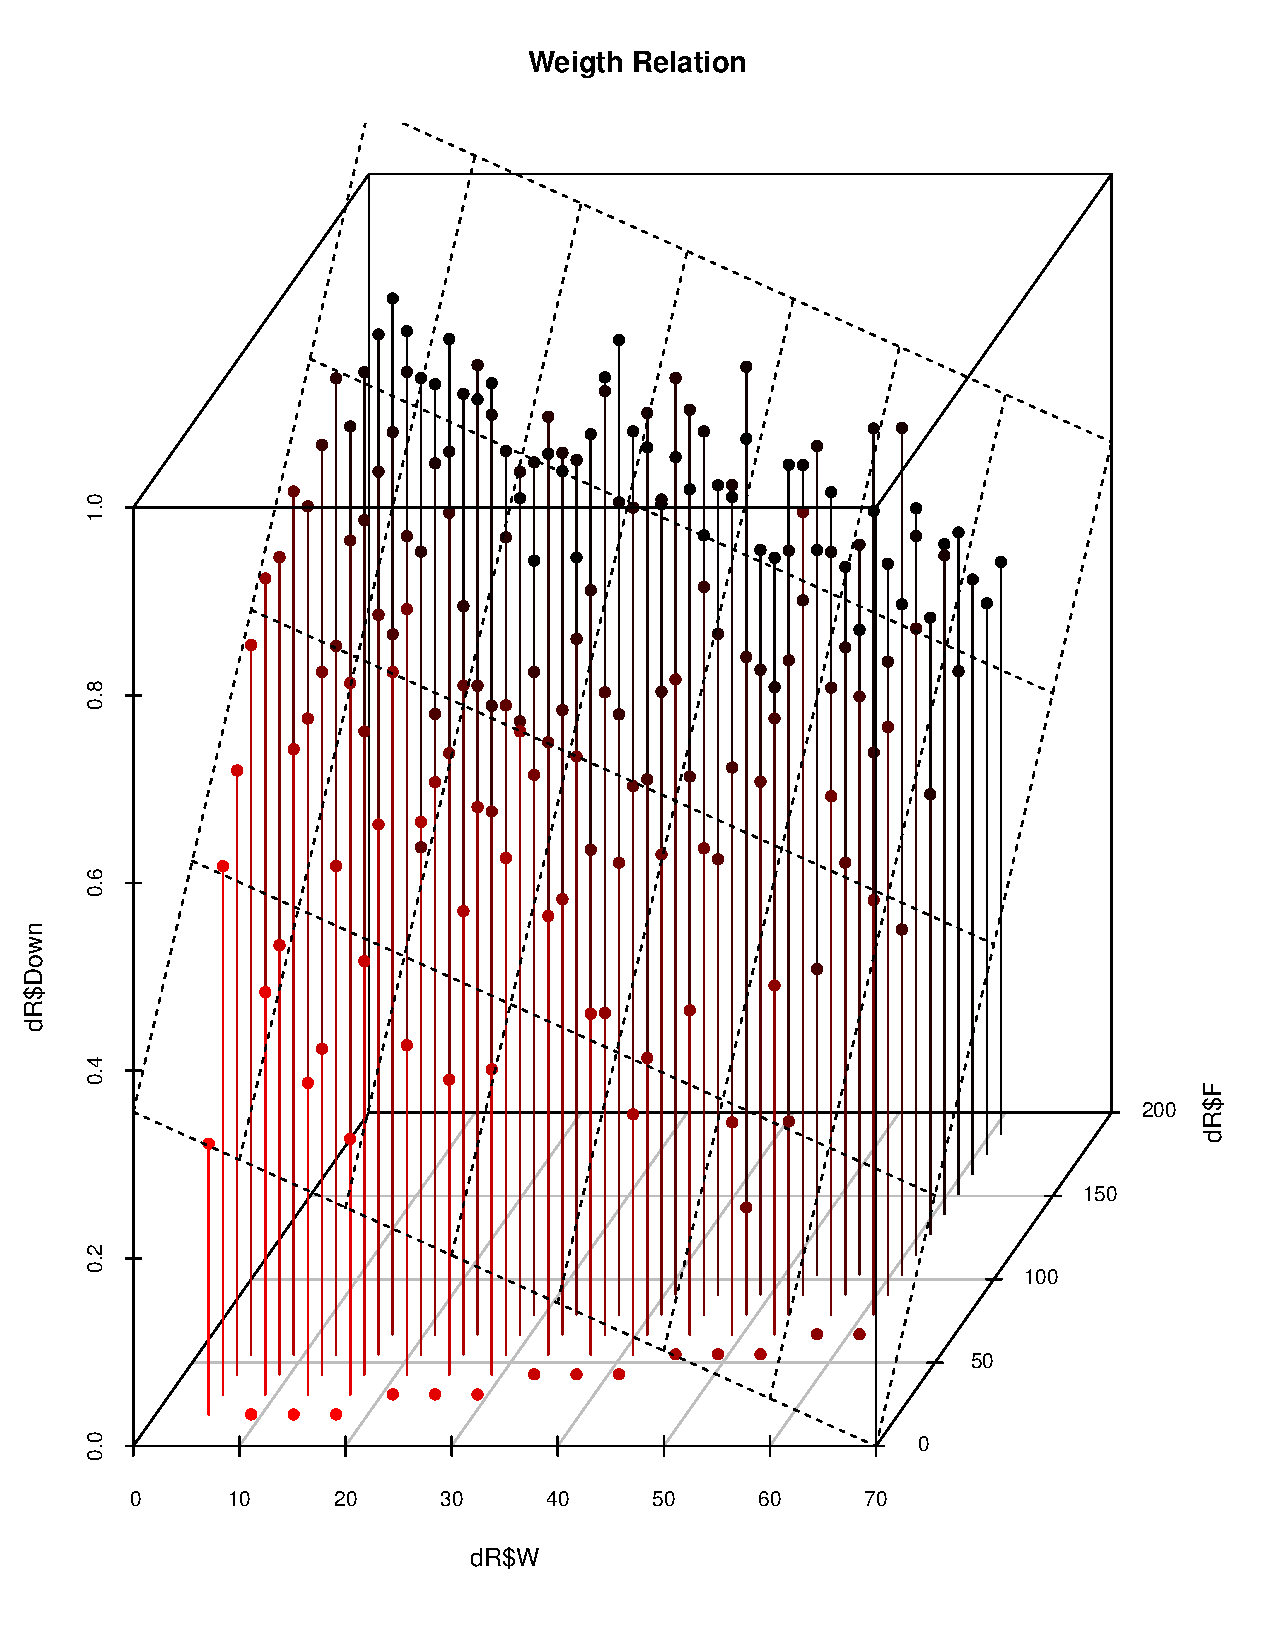
\includegraphics[width=\linewidth]{images/WeightRelationDown}
    \label{fig:WeightRealtion}
  \end{subfigure}
  \caption{Heatmap of Relation between size of weight matrix $W$ and focal matrix $F$}
  \label{fig:RealtionDown}
\end{figure}
\subsection{Clumping}

\subsection{Zoom}

Blueline is Focal $G^*$. Redline is $G^*$

\begin{figure}[htp]
  \begin{subfigure}{\linewidth}
    \caption{Upward}
    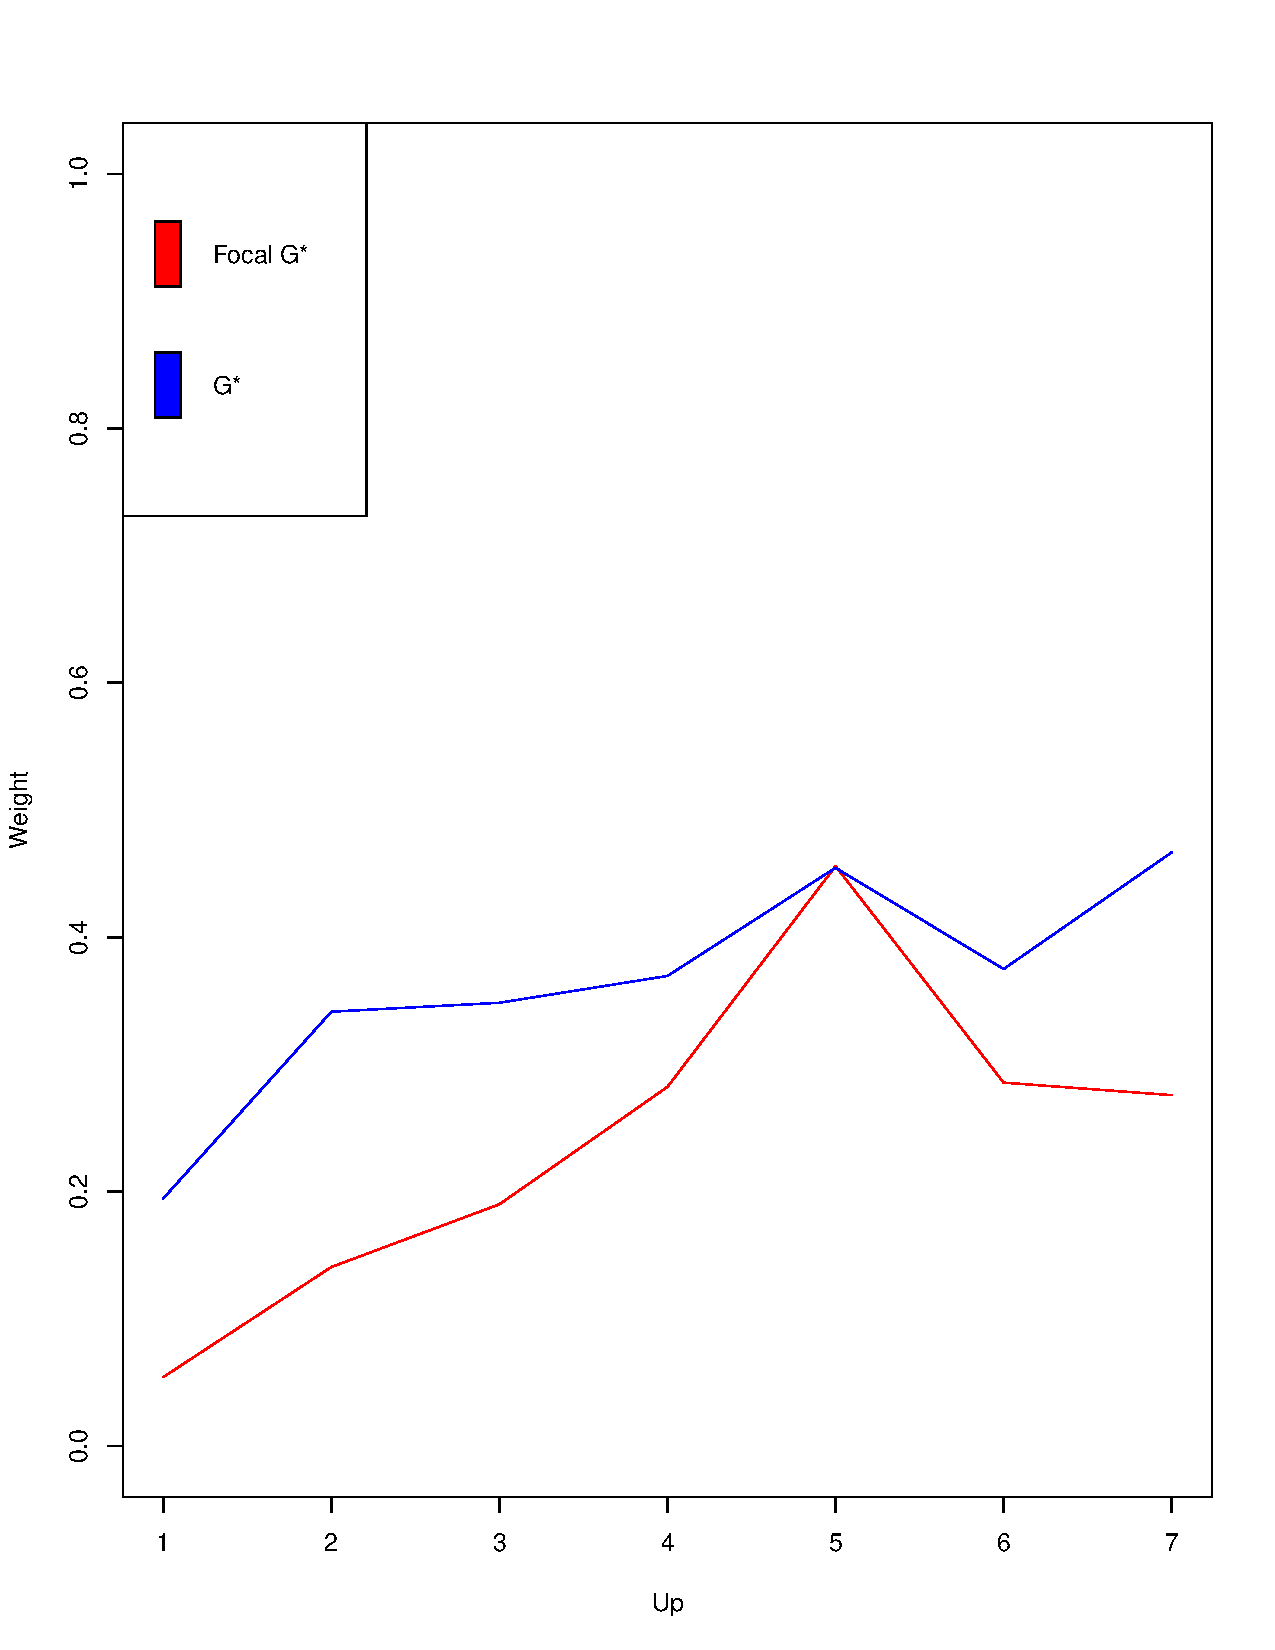
\includegraphics[width=\linewidth]{images/SoHZoomUp}
    \label{fig:UpwardZoom}
  \end{subfigure}
  \hspace{1em}
  \begin{subfigure}{\linewidth}
    \caption{Downward}
    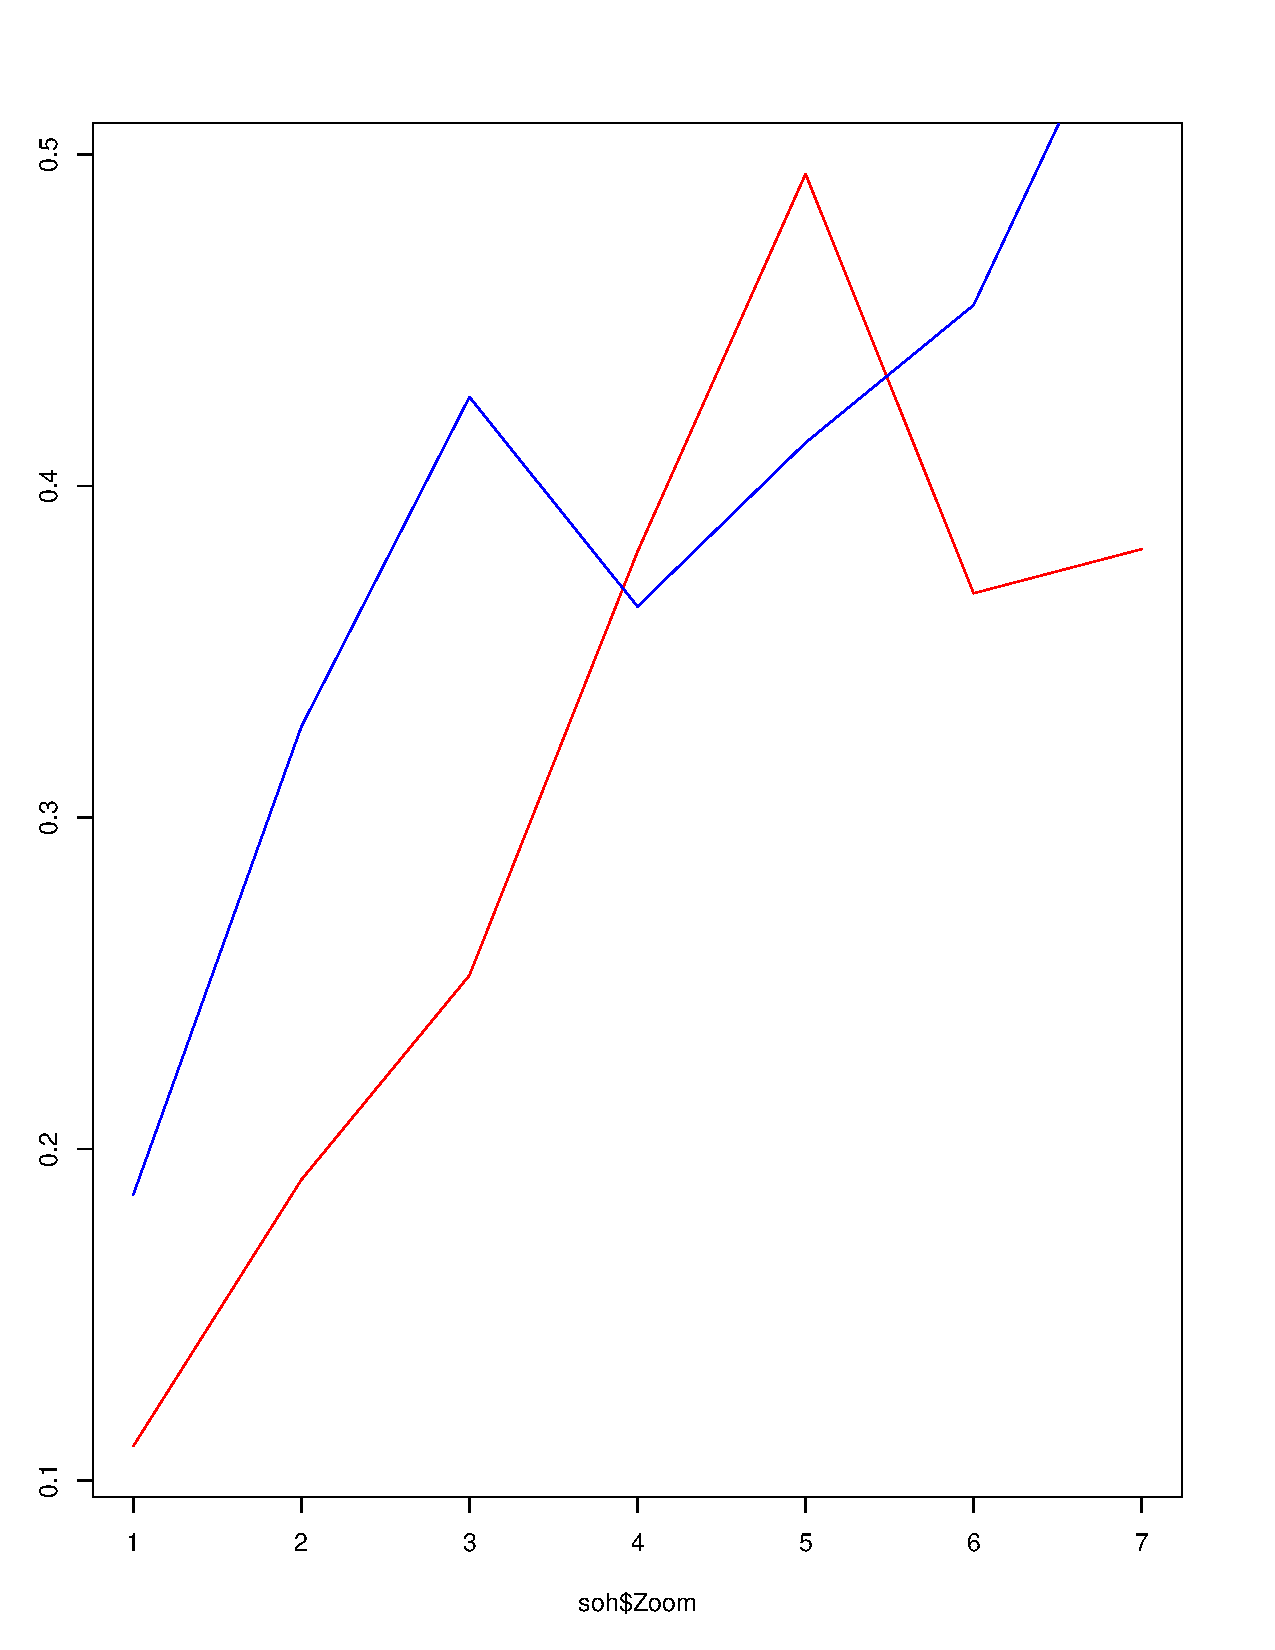
\includegraphics[width=\linewidth]{images/SoHZoomDown}
    \label{fig:DownwardZoom}
  \end{subfigure}
  \caption{TODO}
  \label{fig:Zoom}
\end{figure}


\subsection{Blur}

\begin{figure}[htp]
  \begin{subfigure}{\linewidth}
    \caption{Upward}
    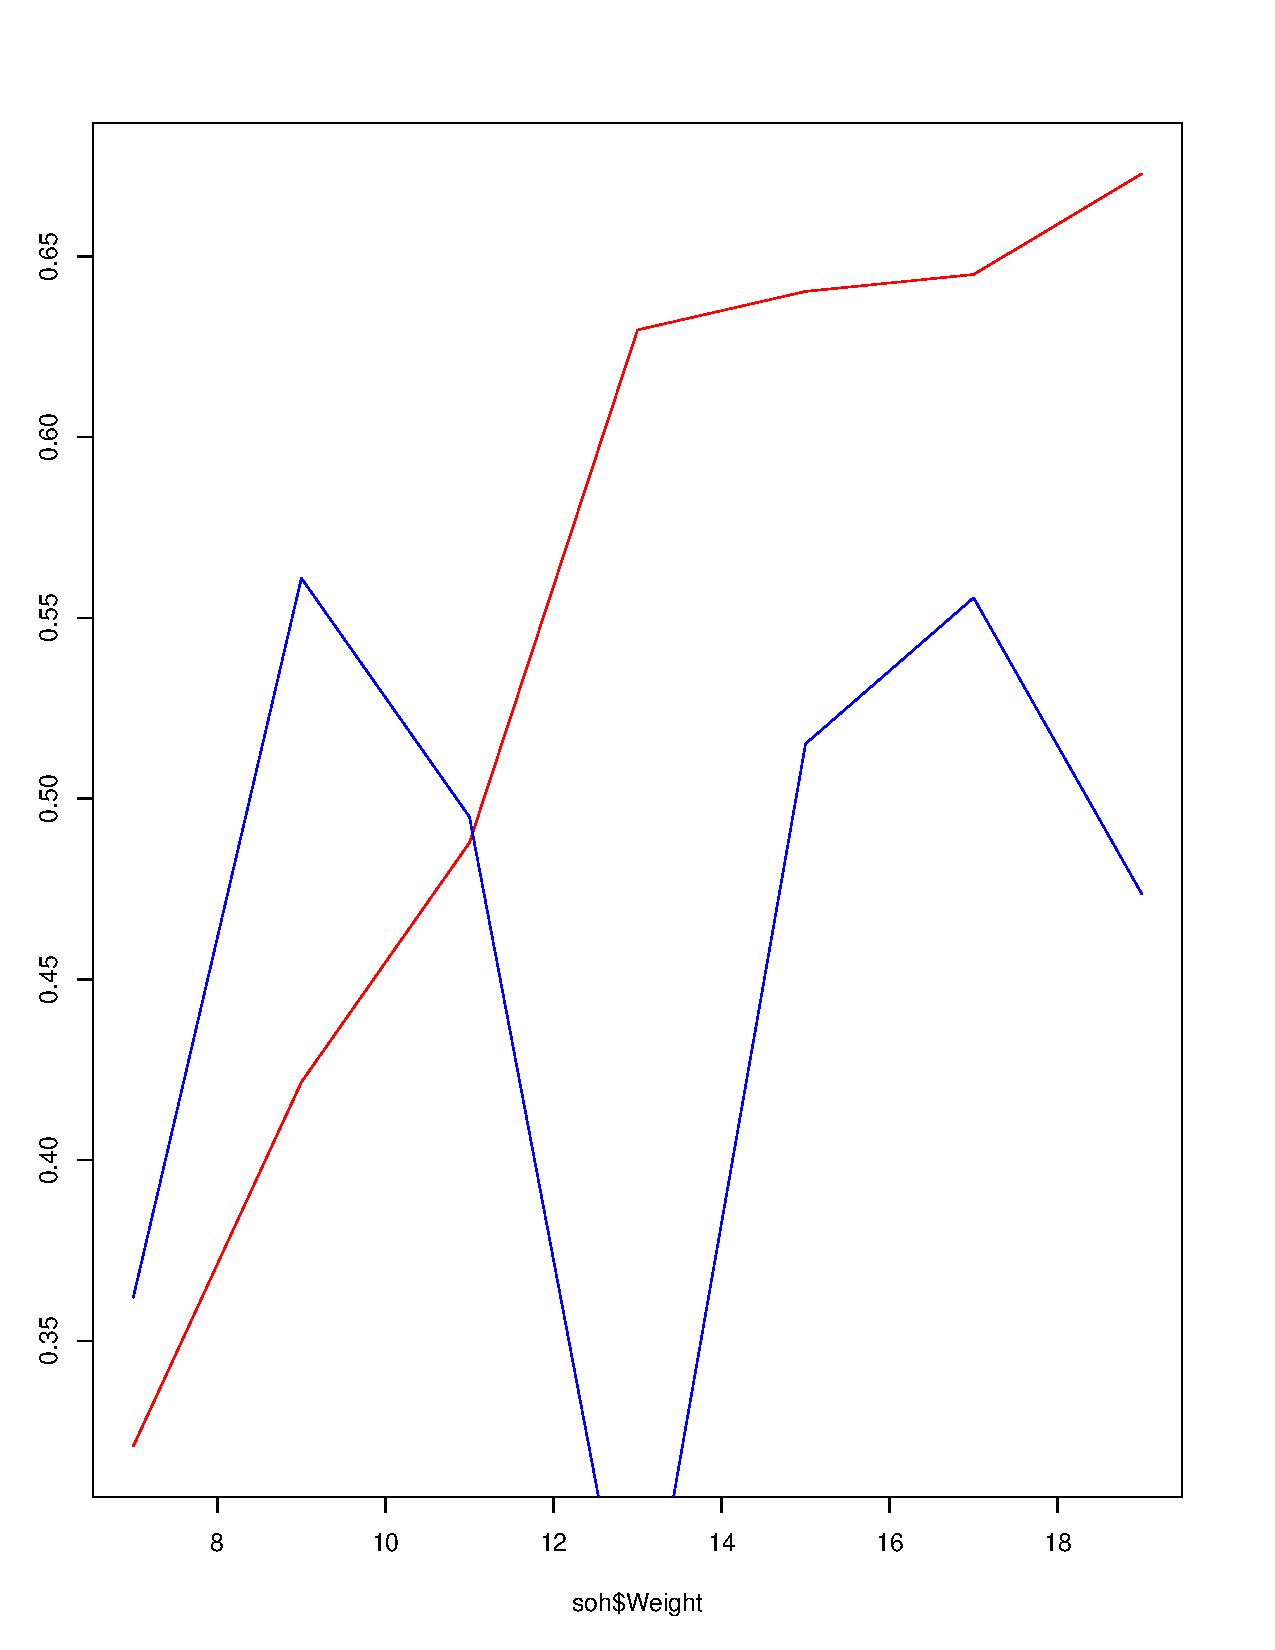
\includegraphics[width=\linewidth]{images/SoHUpBlur}
    \label{fig:UpwardBlur}
  \end{subfigure}
  \hspace{1em}
  \begin{subfigure}{\linewidth}
    \caption{Downward}
    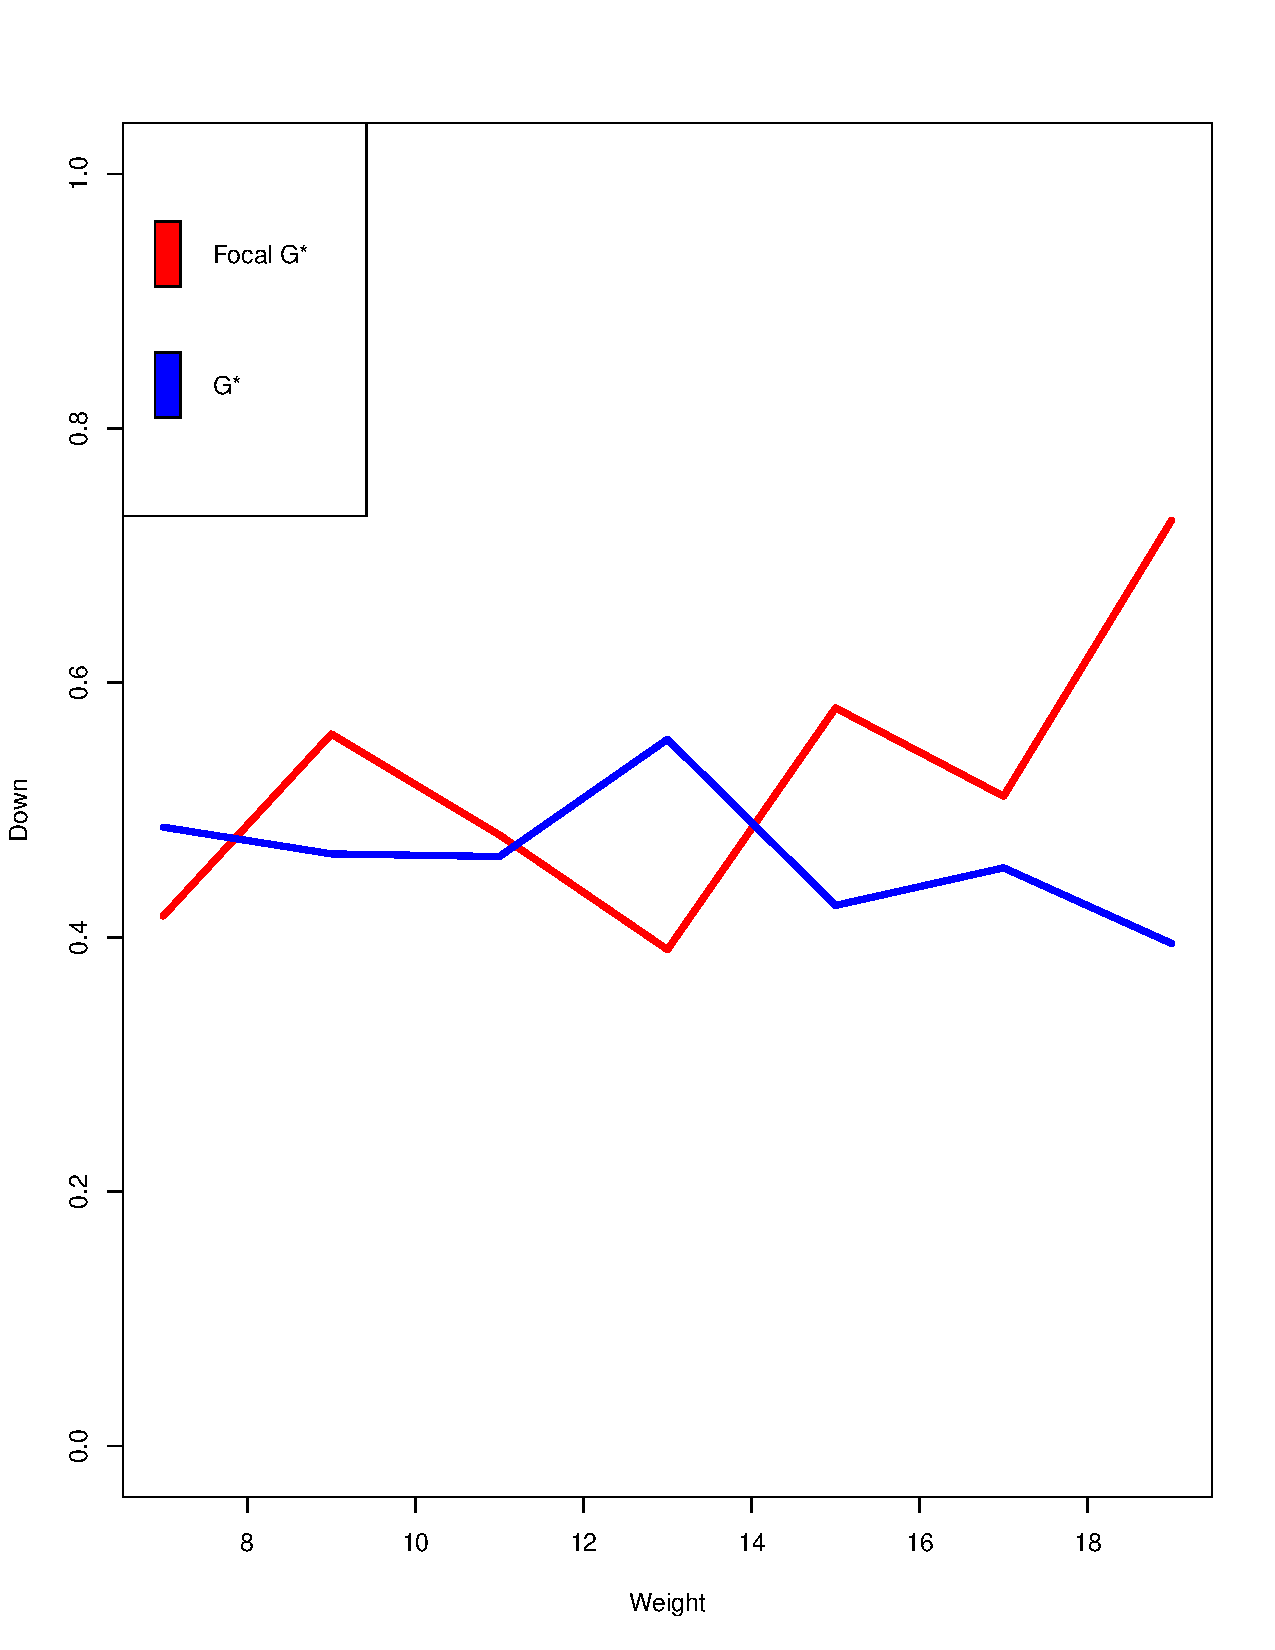
\includegraphics[width=\linewidth]{images/SoHDownBlur}
    \label{fig:DownwardBlur}
  \end{subfigure}
  \caption{TODO}
  \label{fig:Blur}
\end{figure}


\subsection{Results and Discussion}




The results for the hot spot analysis are found in
Fig.~\ref{fig:ComparisonMorning} and Fig.~\ref{fig:ComparisonEvening} for a
comparison of $G^*$ and the Focal $G^*$ statistic. It can easily be seen that
both versions produce similar results, but the focal versions produces a more
differentiated picture for larger weight matrices. Small differences on a
global scale are more pronounced on a regional scale and result in smaller and
finer areas for hot spots. This enables the detection of additional hot spots
and interesting areas which are most easily observable for the weight matrix of
size $7{\times}7$ in the evening (Fig.~\ref{fig:ComparisonEvening}). This
enables the detection of significant deviations from the surrounding area. 
In contrast the Standard $G^*$ statistic shows larger areas as important.
Therefore, depending on the need of a planner, the Focal $G^*$ statistic
is more helpful to identify individual areas of interest whereas the standard
$G^*$ statistic gives a more broad overview. For the identification of IUHI this
is quite important. As a city planer wishes to detect critical areas, it is
important to detect not only general hot areas, but also those points where the
most extreme differences in a local context exist. Finding those areas can help 
identify the underlying reasons or plan individual solutions.

Based on these images one can also see that the hot spots found by the Focal
$G^*$ statistic seem to be more stable. We compare their stability using only
the $ SoH^\uparrow$ for lack of space. A plot of the results can be found in
Fig.~\ref{fig:EvalResults}. Fig.~\ref{fig:EvalResults} compares the $
SoH^\uparrow$ between each increasing size of the weight matrix W. At a first
glance, one can see that the typical implementation with a square weight matrix
is the most unstable hot spot analysis, regardless of time of day. This is to be
expected as the binary weights increase the dependence on the weight matrix. The
use of a decreasing weight matrix perform better. As the more outlying data
points get less weight, this reduces the dependence on the weight matrix and
leads therefore to more stable results. Our proposed Focal $G^*$ statistic
achieves the most stable results in almost all cases. Only data points in a
restricted region around the area of interest may influence the significance
result. Through this restriction high values at key points gains more weight
regardless of the weight matrix and are therefore more independent of the weight
matrix. This increases the stability. The decrease in stability for the largest
weight matrices is most likely a result of the parametrization of the focal
matrix. With increasing size of the weight matrix in relation to the focal
matrix the value of each pixel is approaching to the mean of the area of the
weight matrix. As can be easily seen from Def.~\ref{def:GenericGetisOrdFunc}
then the value for every pixel would be zero.

\section{Conclusions and Future Work} \label{sec:Conclusion}

In this work, we generalized the Getis-Ord statistic to deal with the problem of
stability inherent in hot spot analysis. We identified possible underlying
reasons for this instability: The weight matrix as well as the size of the study
area. We developed a modified approach that deals with those two factors. The
result is a modified $G^*$ statistic called the \emph{Focal $G^*$ statistic}. It
reduces the study area used for comparison into regions and achieves through
this an increase in stability. To determine the effectiveness of our approach,
we propose a stability metric for hot spots called \emph{SoH}. To our knowledge
no such metric existed before this work. The SoH computes the ratio of
dependence of hot spots for different parametrizations of weight matrices. It
enables to express the stability between each parametrization using single value
restricted between zero and one. Based on this number one can decide which
parametrization to use and researchers can compare the stability of their
methods for unsupervised hot spot analyses. In particular, for temperature
values one wishes to detect those areas which have high differences regardless
of a particular parametrization. If a hot spot only appears for one
parametrization, the information gained for general use is quite small and can
even lead to an inefficient allocation of resources.

This research has several restrictions which have to be taken into account.
First, we only tested the $SoH^\uparrow$ metric. While we assume, based on our
graphical analysis, that the  $SoH^\downarrow$ stability should be similar, we
have no hard results. The results themselves are tested on two events in time
for a fixed area of the city of Karlsruhe. We have not tested it on smaller or
larger study areas, but we assume that the stability of the Focal $G^*$ would
stay the same whereas the stability of the $G^*$ statistic would increase with a
smaller study area and decrease with a larger study area. This follows the
reasoning that the impact of a singular point increases with a decrease of the
study area. To test this dependency is an interesting task for future work. The
last restriction is the fixed size in this work of the focal matrix for the
Focal $G^*$ approach. We only tested one size in this work, but it is highly
probable that the size of the focal matrix has an impact on the stability as
could be seen in Fig.~\ref{fig:EvalResults}. While an overall trend can be seen
in this work when the size of the weight matrix W and the focal matrix F are
almost identical, the exact ratio is beyond the scope of this work. The optimal
ratio as well as when the stability suffers from a too similar size are
interesting question for future work.

\section{Acknowledgements}
This work is part of the research project BigGIS (reference number: 01IS14012)
funded by the Federal Ministry of Education and Research (BMBF) within the
frame of the programme "Management and Analysis of Big Data" in "ICT 2020 --
Research for Innovations".
We thank the Nachbarschaftsverband Karlsruhe for the data of the thermal flight
over Karlsruhe. %
\noindent R-packages used: \verb|raster|~\cite{cran:raster}, 
\verb|knitr|~\cite{cran:knitr}

\bibliographystyle{plain}
\bibliography{bibfile}  % sigproc.bib is the name of the

\end{document}
